%!TEX root = ../main.tex
\chapter{Simulation and Software tools}
\label{chap:G4Simulation}

In high energy physics as well as in other research areas, simulations are a tool that has become indispensable. They are used to provide model predictions, a guideline for an analysis as well as for optimizing cost and performance of detector designs. In this thesis, the simulations will be used as a guideline for the selection of specific events of the recorded data. An understanding of their functioning is useful and will be described in section \ref{sec:SimModels}. The software tools and the \ilcsoft framework used for this analysis will be described in section \ref{sec:Software}. Finally, the AHCAL simulation model and the digitization procedure will be discussed in section \ref{sec:AHCALGeometry}.

\section{Simulation of particle showers}
\label{sec:SimModels}

The \geant framework \cite{Agostinelli2003} is a common toolkit in particle physics to simulate particle interactions with matter for a wide range of energies. Within this thesis, the simulations of the CALICE calorimeter prototypes and the ILD detector concept are used in conjunction with the \mokka \cite{Freitas2003} and \ddhep \cite{Frank2014} framework. These frameworks provide a variety of tools for the implementation of detector geometries. \geant offers various tools and models to simulate physics processes in particle showers.

\subsection{Electromagnetic shower models}

Electromagnetic showers are generally well understood. This is mainly due to the fact that only electrons, positrons and photons are involved and their interaction with matter is simple as described in section \ref{sec:PartInter}. All EM interactions are simulated with a standard EM package in \geant \cite{Ivanchenko2010}. This package has been extensively compared to many observables measured in calorimeters to a level of $\leq$ 1\% \cite{Apostolakis2015}.

Recently additions have been made to the \geant EM physics list by improving the description of ionization processes in the active medium. Then the EM list is used with a suffix \_{}EMY. This is needed in order to correctly simulate thin active layers where the detection method is very sensitive to the primary ionization, like in gas detectors such as RPCs. The use of the \_{}EMY suffix in the EM physics list is greatly improving the agreement between data and simulation in the RPC based CALICE calorimeter prototypes, the SDHCAL and DHCAL \cite{Neubueser2016}. Many other suffix options are available depending on the type of physics, detector and precision needed for EM processes.

\subsection{Hadronic shower models}

Hadronic showers are more complex in many ways than EM showers mainly due to the compositeness of the projectile as well as the target nucleus. High energy interactions between these lead to a very large phase space in the final state. The interaction is governed by the strong force and generally cannot be solved analytically. Instead, models are used using approximations and parametrizations mainly derived by theory and matched to data. Significant work has been made in the last few years in improving the modelization and accuracy of such models. The CALICE Collaboration has been of a great help in contributing to these improvements \cite{Adloff2013, Bilki2015}.

The scale of the interaction in hadronic showers is generally given by the De Broglie wavelength $\lambda_{B} = h/p$. This simple variable becomes shorter as the particle energy increases thus smaller structures inside a nucleus become more relevant for the description of the interaction. \geant provides several models that are valid over various energy ranges. These models are described in the following.

\subsubsection{Intra-Nuclear Cascade Models}

For particle energies above a few hundred MeV and below a few GeV, the quark substructure of the nucleus is irrelevant. In this case, the interaction can be described by intra-nuclear cascade models (see figure \ref{fig:cascademodel}). Several models are available in \geant and will be described in the following.\\

\begin{figure}[htbp!]
  \centering
  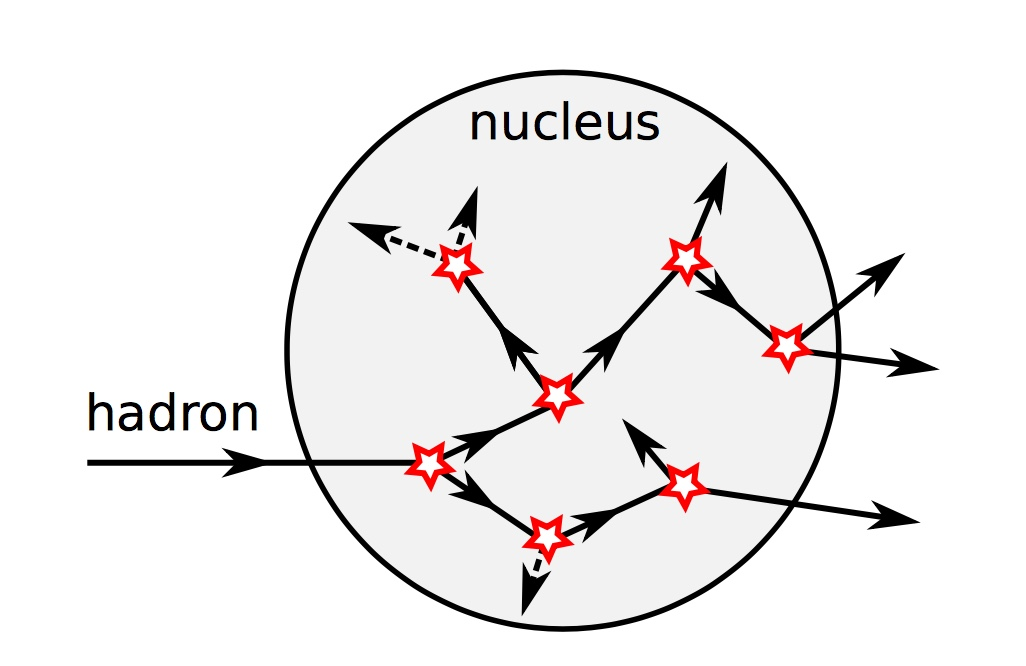
\includegraphics[width=0.5\linewidth]{chap4/fig/CascadeModel.jpeg}
  \caption{Schematic of the cascade model. The incoming projectile and all secondaries inside the nucleus are tracked and their interaction is calculated until their energy is under a certain threshold or leave the nucleus \cite{Feege:2011dsa}.} \label{fig:cascademodel}
\end{figure}

\textbf{Bertini Cascade}\\

The Bertini cascade model \cite{Heikkinen2003} consists of the modeling of a nucleus by three concentric spherical shells of approximately constant nucleon density. The nucleons are treated as a degenerated Fermi gas in each shell and all energy levels are filled up to the Fermi energy ($E_F$). Following the Pauli exclusion principle that products can't be in an occupied state (lowest level filled by the Fermi gas), only secondary nucleons of energy $E > E_F$ can be produced. During the intra-nuclear cascade (INC), the momentum, the type of interaction and the four-momenta of the interaction for each nucleon are calculated until the energy of the tracked nucleon is below 2 MeV. The INC gives rise to excited states of the nucleus and a pre-equilibrium evaporation is computed (emission of proton and neutrons). Then a de-excitation model is applied including Fermi break-up of highly excited light nuclei (A < 12), explosion model, fission model and evaporation model until the excitation energy is below 0.1 MeV.\\

\textbf{Binary Cascade}\\

The Binary cascade \cite{Folger2004} is another approach to model the interaction between a projectile and a target nucleus. The model describes the nucleons with defined position and momentum following the nucleus mass, density distribution and Pauli's exclusion principle. The momentum is chosen randomly between zero and the Fermi momentum ($p_{F}^{max}(r)$) such that the total momentum of the nucleus is zero (at rest). The model is then treated by steps of excitations and decay into secondary particles emerging from the interaction until the average energy of all participants in the nucleus is below a given threshold (70 MeV). The remaining nucleus is further treated by pre-equilibrium and de-excitation models in \geant. The validity range of this model extends from around 100 MeV up to 10 GeV.

\subsubsection{String-Parton Cascade Models}

\begin{figure}[htbp!]
  \centering
  \begin{subfigure}[t]{0.49\textwidth}
    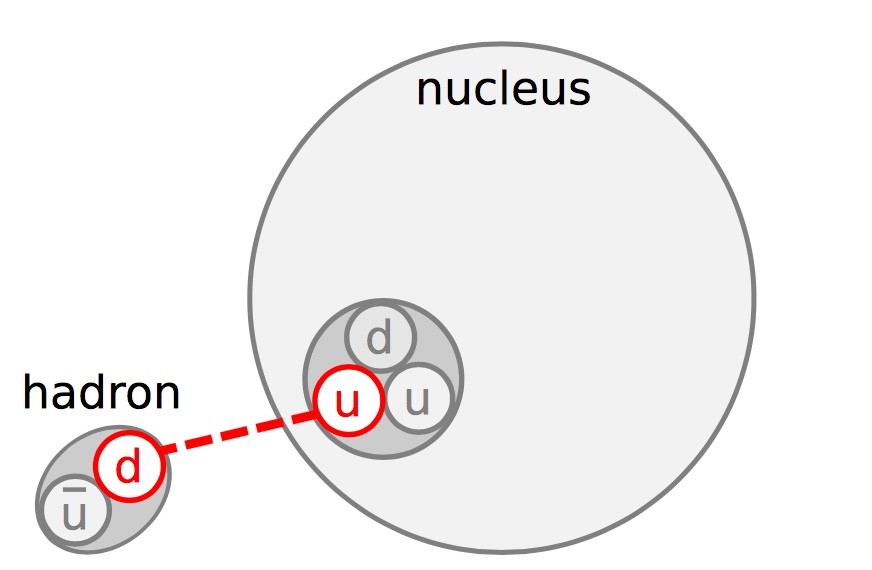
\includegraphics[width=1.\linewidth]{chap4/fig/QGS_nucleus.jpeg}
    \caption{} \label{fig:QGS_nucleus}
  \end{subfigure}
  \hfill
  \begin{subfigure}[t]{0.49\textwidth}
    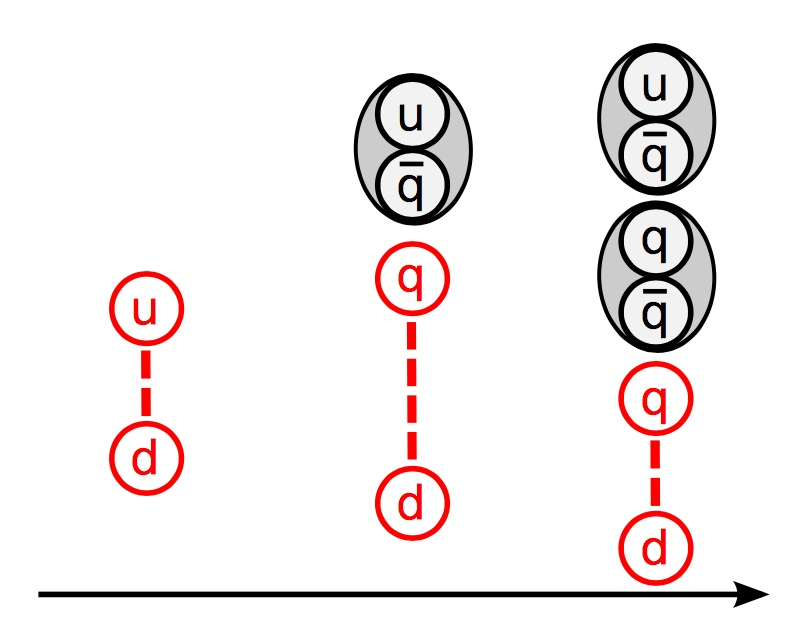
\includegraphics[width=1.\linewidth]{chap4/fig/QGS_stringfrag.jpeg}
    \caption{} \label{fig:QGS_string}
  \end{subfigure}
  \caption{\subref{fig:QGS_nucleus}) The sketch shows the formation of a string between the projectile and one of the quarks inside the nucleus. \subref{fig:QGS_string}) Representation of the fragmentation of the strings via the generation of quark-antiquark pairs into hadrons \cite{Feege:2011dsa}.}
\end{figure}

The string-parton models \cite{Folger2003} are used in \geant to simulate inelastic scattering of particles with a target nucleus as shown in figures \ref{fig:QGS_nucleus} and \ref{fig:QGS_string}. This is used at high energies where INC models break down and where the quark substructure of the nucleons must be taken into account. The model uses string excitation to calculate the scattering. Currently, \geant provides two different models, the Fritiof model (FTF) and the quark-gluon string model (QGS).

The initial state consists of building the nucleus of individual protons and neutrons. The interaction between the primary particle and the nucleus gives place to one or more excited strings and an excited state nucleus. Quarks are the interacting constituents in the primary particle and the nucleons of the target nucleus. A string has two endpoints, such that the quark content is defined and carries energy and momentum. The fragmentation of the strings is handled by a longitudinal string fragmentation model and the interaction of secondaries is carried out by cascade models as described in the former paragraph. The de-excitation is then simulated by fragmentation, pre-compound and nuclear de-excitation models natively provided by \geant. The QGS model uses longitudinal strings to represent the momentum transfer and transverse strings for color exchange via Pomerons. In contrary, the FTF model uses an interaction probability calculated based on impact parameter, the center of mass energy, diffractive and elastic cross-sections to form a string. In the next paragraph, the QGS and FTF models are called QGSP and FTFP respectively.

\subsection{\geant Physics Lists}

\geant provides several physics lists for simulation that combine different hadron physics models. The physics lists are combinations of models, active in different energy ranges \cite{Geant4PhysicsLists:IEEE}. In this thesis, the physics lists QGSP\_BERT and QBBC are used. The validity range of the physics lists is shown in figure \ref{fig:physics_list}. The former is used in combination with the High-Precision neutron tracking (HP) package. The HP option delivers an increased accuracy in the treatment of neutron interactions below 20 MeV. The QBBC physics list includes also a tracking for neutrons with less precision than the HP package.
In addition, the QGSP\_BERT physics list uses a parametrized LEP model (based on experimental data) to fill the gap between the transition of cascade models and string-parton models.

\begin{figure}[htbp!]
  \centering
  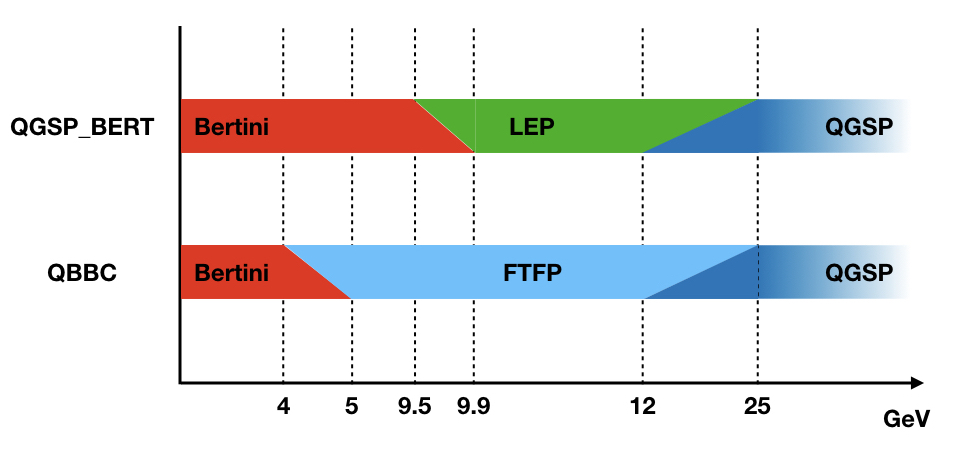
\includegraphics[width=1\linewidth]{chap4/fig/PhysicsLists.jpeg}
  \caption{Schematic of the physics list used in \geant v10.1 for this thesis. The validity range extends above 30 GeV. The diagonal regions represent the overlap region between the different models. The probability to select each model varies linearly between 0 and 100\% in the overlap region.} \label{fig:physics_list}
\end{figure}

\section{Software tools}
\label{sec:Software}

\subsection{\ilcsoft software framework}

Various tools developed by the Linear Collider community are grouped in a common software framework called \ilcsoft \cite{ILCSoftPortal}. It provides a complete framework that can be used for Monte-Carlo studies and experiments. As an example, physics studies, ILD detector optimization and performance for the ILC are performed within the \ilcsoft framework.\\

Most of the tools in the framework use an Event Data Model (EMD) named Linear Collider I/O (\lcio) which provides a reliable and performant solution for simulation and analysis studies \cite{Gaede:2003ip}. With this tool, various detector concepts and analysis can be shared between collaborations such as SiD, ILD, CLIC, FCC.

The \ilcsoft framework provides a modular \cpp framework named \marlin for reconstruction and analysis of physics events \cite{Gaede:2006pj}. \marlin uses \lcio seamlessly and is configured using XML steering files. \marlin enables users to develop custom modules for their own and run it along with other already existing modules.

The reconstruction and analysis tools used in this analysis are mostly part of \ilcsoft. For this thesis, \ilcsoft v01-17-11 was used for simulation, reconstruction and analysis.

\subsection{CALICE software framework}

The CALICE collaboration has developed, since the physics prototypes, a software framework used for the simulation, digitization of simulated data and the calibration of the testbeam data using the \marlin framework. For this thesis, a software development version (v04-08-03) was used and is available on the DESY svn server \cite{CALICESoft, 6036245}.

\section{AHCAL Detector Geometry implementation and Digitization}
\label{sec:AHCALGeometry}

\subsection{Geometry implementation}

The simulation of the testbeam prototype presented in this thesis (see chapter \ref{chap:EvtSelection}) is based on the \mokka \cite{MoradeFreitas:2002kj} framework v08-05-01 and the new \ddhep \cite{Frank:2014zya} framework v00-16, which both provide a full \geant v10.1 based simulation of the detector with detailed geometry and material descriptions. A right-handed coordinate system is used such that the Z-axis points in the beam direction and that the Y-axis is directed upwards. No beamline instrumentation is simulated except scintillator triggers in front of and behind the detector. An additional layer of 5.6 mm of lead (corresponds to 1 $X_0$) is added in front of the calorimeter in order to account for missing upstream material. This additional material was determined using the electron data and matching the simulation with the center of gravity distribution in the z-direction (see appendix \ref{appendix:SimulationVal}).

This analysis uses the sub-detector \mokka models \textit{TBecal4d} for the ScECAL (Scintillator strips with EBUs) and \textit{TBhcal4d} for the AHCAL. The distance between the sub-detectors is set to 0 mm. The absorber structure is square-shaped in simulation, on contrary wedge-shape in reality, but it is not expected to have any influence. The placement of the active layers are the following: 2 single EBU boards, 8 single HBU boards and 4 $2\times2$ HBU boards (in slots 11, 13, 21, 31 of the absorber structure). A schematic can be seen in figure \ref{fig:Det_layout}.
\begin{figure}[htbp!]
  \centering
  \begin{subfigure}[t]{0.59\textwidth}
    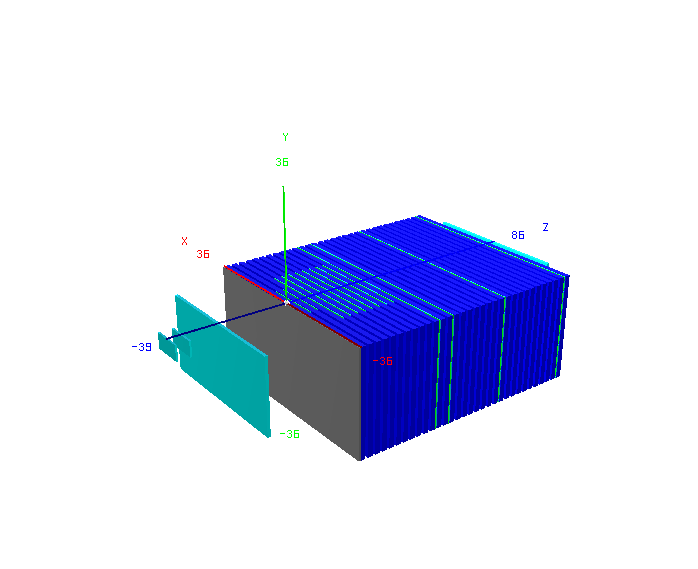
\includegraphics[width=1.\linewidth]{chap4/fig/DD4hep_AHCALModel.png}
    \caption{} \label{fig:GeomModel}
  \end{subfigure}
  \hfill
  \begin{subfigure}[t]{0.39\textwidth}
    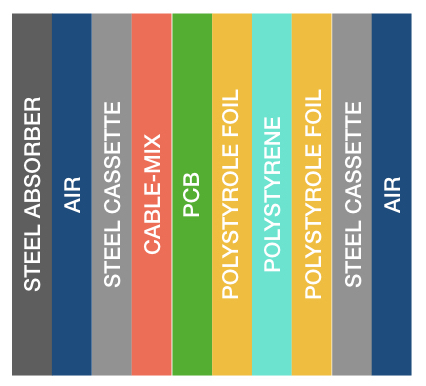
\includegraphics[width=1.\linewidth]{chap4/fig/Structure.jpeg}
    \caption{} \label{fig:material_layout}
  \end{subfigure}
  \caption{\subref{fig:GeomModel}) DD4hep geometry model of the 2015 testbeam prototype. The dark blue represents the steel absorber structure, the light blue represents the active scintillator layers and the beam instrumentation in front and back of the calorimeter and the dark grey represents the additional lead material to account for missing upstream material. \subref{fig:material_layout}) Material description of one layer in the \mokka and \ddhep simulations of the AHCAL. Dimensions are not to scale.}
\end{figure}

The material description is showed in table \ref{table:material_sim} for thicknesses and corresponding radiation length and nuclear interaction length. A schematic of the HCAL layer structure can be seen in figure \ref{fig:material_layout}. The cable-mix of 1.5 mm, the polystyrole foils of 0.115 mm and the air gaps of 1.285 mm are not listed because of the negligible impact but are present in simulations. A picture of the model in \ddhep is shown in figure \ref{fig:GeomModel}. The simulation includes also saturation effects in the scintillator known as the Birk's Law. The saturation appears a high ionization densities due to shielding effects of the scintillator material. The implementation of the Birk's Law in \geant is used and follows the expression
\begin{equation}
  \frac{dL}{dx} = \frac{dE}{dx} \times \frac{1}{1 + k_B \frac{dE}{dx}}
\end{equation}
with $\frac{dL}{dx}$ the light yield by unit length and $\frac{dE}{dx}$ the ionization density. The parameter $k_B$ depends on the material and a value of 0.07943 mm/MeV is taken \cite{kB:IEEE}.
A check was performed with \mokka and \ddhep models with muons and electrons to ensure that the material description in both models is better than 20\% (see appendix \ref{appendix:SimulationVal}).
\begin{table}[htb!]
  \centering
  \caption{Material description in \mokka and \ddhep simulations of the testbeam setup at CERN in July 2015. The X$_0$ and $\lambda_n$ numbers are obtained by the command-line \textit{materialScan} in the \ddhep framework.}
  \label{table:material_sim}
  \begin{tabular}{@{} p{6cm}|l||l|l @{}}
    \hline
    Material & thickness (mm) & X$_0$ & $\lambda_n$ \\
    \hline
    \hline
    steel absorber & 17.2 & 0.977 & 0.101\\
    \hline
    steel cassette & 0.5 & 0.028 & 0.003\\
    \hline
    PCB & 0.7 & 0.004 & 0.001\\
    \hline
    Polystyrene (ECAL/HCAL tile) & 2, 3 & 0.005, 0.007 & 0.006, 0.009\\
    \hline
    \hline
    ECAL layer & 26.2 & 1.044 & 0.115\\
    HCAL layer & 26.2 & 1.046 & 0.118\\
    \hline
    AHCAL & - & 33.24 & 3.54\\
    \hline
  \end{tabular}
\end{table}

The beam gun is placed 1 m in front of the calorimeter face for the simulations in this analysis. It is configured to generate single beam particles with a 2\% momentum spread, according to the beamline \cite{H2Beamline}, and the beam profile for electrons and pions is extracted from data and applied to simulation. For muon runs, a flat beam covering the full AHCAL is simulated as this is not expected to have an influence on the MIP and time response of the detector. All electron simulations are simulated with \geant v10.1 using the QGSP\_BERT\_HP physics list.

Pion showers are simulated using QGSP\_BERT, QGSP\_BERT\_HP and QBBC physics lists. The package \textit{high precision} (\_HP) is used in order to understand the differences induced in timing with a precise treatment of the neutrons. The table \ref{table:event_sim} shows the number of single particle events simulated for this thesis.

\begin{table}[htb!]
  \centering
  \caption{Number of single particle events simulated in \mokka and \ddhep for each particle type and energy.}
  \label{table:event_sim}
  \begin{tabular}{@{} ccc @{}}
    \hline
    Particle & Energy & \# Events \\
    \hline
    $\mu^-$ & 150 GeV & 1 000 000 \\
    \hline
    $e^-$ & 15, 20, 30, 40 GeV & 20 000 \\
    $e^-$ & 10, 50 GeV & 200 000 \\
    \hline
    $\pi^-$ & 10, 30, 50, 70, 90 GeV & 500 000 \\
    \hline
  \end{tabular}
\end{table}

\subsection{Digitization}
\label{subsec:Digitization}

The digitization of simulated hits is very similar to the one used in the ScECAL and AHCAL physics prototypes \cite{2011_JINST_6_P04003}. First, the energy deposited in a cell is converted in MIP. This is done in order to have the simulation on the same energy scale (see chapter \ref{chap:ECalibAHCAL}) as the testbeam data once converted. The conversion unit named \textit{MIPtoGeV} is extracted from simulation by projecting 8 GeV muons onto the AHCAL detector and fitting the resulting spectrum of the deposited energy. Motivated by physics, as explained in section \ref{sec:PartInter}, ideally for a thin active material, the energy deposited follows a Landau distribution. The most probable value (MPV) of this distribution is used as the \textit{MIPtoGeV} factor. For this thesis, a value of 470 keV is used for the AHCAL as shown in figure \ref{fig:landau_MPV} and 309 keV for the ScECAL.

\begin{figure}[htbp!]
  \centering
  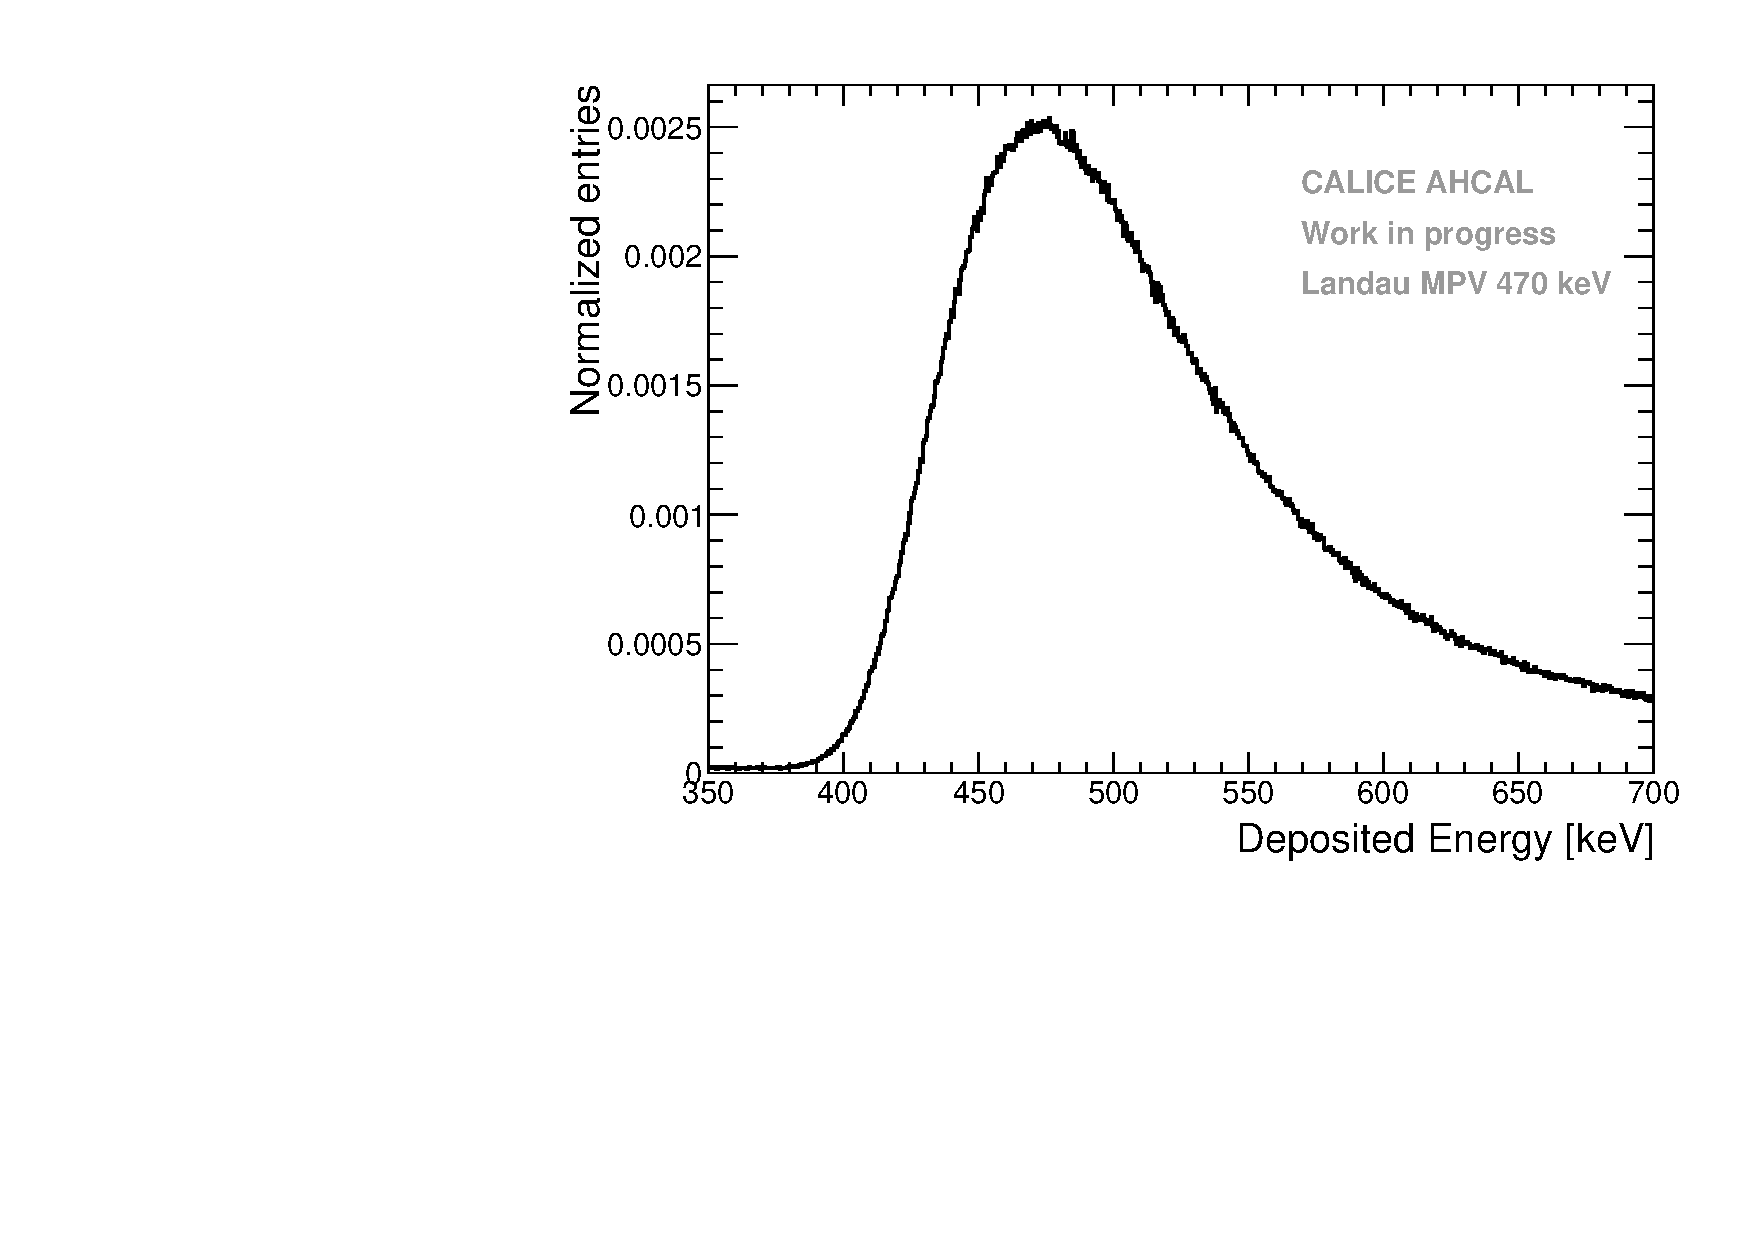
\includegraphics[width=0.5\linewidth]{chap4/fig/Landau_mu_HCAL.pdf}
  \caption{The energy deposited in the AHCAL cells from the raw simulation without any detector effects for 8 GeV muons. The spectrum has been fitted with a Landau distribution and the MPV is extracted as the \textit{MIPtoGeV} factor.} \label{fig:landau_MPV}
\end{figure}

If available, individual calibration factors obtained from data are used to extract the light yield which is needed to model the statistical fluctuations of photons hitting a SiPM \cite{Hartbrich:2016bbz}. Saturation effects are also included using the number of pixels available on each SiPM type. Most of the tiles used are wrapped with a reflective foil such that crosstalk effects between channels can be neglected. For layers with no wrapping, a default value of 15\% cross-talk is applied.

Additionally, noise needs to be taken into account for the engineering AHCAL prototype. It is important to note that noise is much lower than in the physics prototype but it is important to be taken into account for this thesis as timing is very sensitive to low statistics late tails. Noise is added using muon runs by removing found tracks and keeping remaining hits. This is described in appendix \ref{appendix:noise}.

The timing is modeled in the same way as in the SPIROC, the energy from sub-hits in a cell is integrated over a sliding time window of 15 ns, if the energy sum passes the threshold, the time of the simulated sub-hit is used as the time of the hit. In order to simulate detector resolution effects, the time of a hit is smeared with a double Gaussian function with slightly different means and sigmas convoluted with a Gaussian of fixed mean and variable sigma. More details are explained in appendix \ref{appendix:ped_shift}.

After digitization, simulated hits have the same format as raw data hits and are then reconstructed using the same software chain as is used for data. To suppress noise, only hits above 0.5 MIP are considered in this analysis in both simulation and data.

\begin{center}
  \rule{0.5\textwidth}{.4pt}
\end{center}

In this chapter, the inner details of the simulation models used for this thesis are discussed. The simulation model of the AHCAL is described in details as well as the digitization procedure of simulated AHCAL hits.

Before taking data in testbeam, the detector has to be commissioned. This means that each channel of the detector has to be characterized in terms of the voltage applied on the SiPM, the SiPM gain, the trigger threshold position and the noise of the detector. In the next chapter, the commissioning procedure of the AHCAL is presented.
